\documentclass{article}
\usepackage{graphicx} % Required for inserting images
\usepackage{float}


\title{Raport AP2}
\author{Chiriac Laura-Florina și Bindiu Ana-Maria }
\date{Ianuarie 2025}

\begin{document}

\maketitle

\section*{Introducere}

În cadrul acestui studiu, am analizat un set de date disponibil la adresa specificată, care descrie informații turistice relevante, incluzând următoarele atribute: \textbf{Location}, \textbf{Country}, \textbf{Category}, \textbf{Visitors}, \textbf{Rating}, \textbf{Revenue}, și \textbf{Accommodation\_Available}. Scopul principal este de a propune o soluție bazată pe algoritmi de Învățare Automată, care să determine o ierarhie optimă a categoriilor de activități tematice (ex.: \textit{Nature, Historical, Cultural} etc.) ce maximizează profitul (\textbf{Revenue}) și/sau profitul per vizitator (\textbf{Revenue/Visitors}) pentru o anumită țară.

\subsection*{Analiza setului de date}
Setul de date conține informații despre locații turistice din mai multe țări, fiecare fiind asociată unei categorii tematice și unui număr de vizitatori. Aceste caracteristici sunt completate de atribute adiționale precum ratingul locației și disponibilitatea cazării. Caracteristicile precum \textbf{Revenue} și \textbf{Visitors} au fost identificate ca fiind cheie pentru rezolvarea problemei, întrucât profitabilitatea unei activități tematice depinde în mod direct de acestea. În plus, atributele categorice precum \textbf{Country} și \textbf{Category} sunt relevante pentru modelarea problemei.

\subsection*{Corelații între variabile}
Atributele numerice precum \textbf{Revenue}, \textbf{Visitors} și \textbf{Rating} sunt analizate pentru a identifica relații potențiale. Spre exemplu, creșterea numărului de vizitatori ar putea avea o influență pozitivă asupra veniturilor, iar tipul de activitate poate avea un impact semnificativ asupra profitabilității. Utilizarea tehnicilor grafice precum histogramele și hărțile de corelație oferă o perspectivă asupra modului în care caracteristicile sunt legate între ele.

\subsection*{Metodologia propusă}
Pentru a rezolva această problemă, se va implementa un algoritm de Învățare Automată care să efectueze predicții bazate pe caracteristicile disponibile. Alegerea algoritmului va fi justificată pe baza unei analize comparative între metodele studiate, luând în considerare performanța lor în cadrul problemei de regresie propuse.

Se vor analiza următorii algoritmi:
\begin{itemize}
    \item \textbf{ID3 (arbore de decizie)} - un model interpretabil, capabil să determine relațiile dintre caracteristicile categorice și numerice.
    \item \textbf{AdaBoost} - o metodă avansată de boosting care poate îmbunătăți precizia prin combinarea mai multor modele slabe.
    \item \textbf{kNN (K-Nearest Neighbors)} - un algoritm simplu și intuitiv pentru estimarea profitului pe baza vecinilor similari.
    \item \textbf{Logistic Regression} - pentru clasificarea auxiliară a categoriilor în funcție de profitabilitate, dacă este necesar.
\end{itemize}

Rezultatele experimentale vor include evaluări comparative pe baza unor metrici precum eroarea medie pătratică (MSE), acuratețea și scorul $R^2$, iar concluziile vor servi la stabilirea unei ierarhii finale a categoriilor de activități.

\section*{Motivarea alegerii algoritmilor}

În cadrul acestui studiu, am selectat algoritmi din paradigma de \textbf{învățare supervizată}, având în vedere natura problemei, care necesită predicția unei valori numerice (\textit{Revenue} sau \textit{Revenue/Visitors}) și ierarhizarea categoriilor de activități tematice. Alegerea algoritmilor s-a bazat pe capacitatea lor de a rezolva probleme de regresie și clasificare, precum și pe performanțele lor dovedite în contexte similare.

\subsection*{Algoritmii selectați}
\begin{itemize}
    \item \textbf{ID3 (arbore de decizie)}: Am selectat acest algoritm datorită capacității sale de a lucra atât cu date numerice, cât și categorice, și de a oferi modele interpretabile. ID3 poate evidenția relațiile dintre caracteristici precum \textit{Country}, \textit{Category} și profit, ceea ce îl face potrivit pentru analiza problemei.
    \item \textbf{AdaBoost}: Am inclus AdaBoost datorită performanțelor sale ridicate în probleme de regresie și clasificare, având capacitatea de a combina modele simple pentru a obține rezultate mai precise. AdaBoost este deosebit de util în captarea relațiilor complexe dintre variabilele din setul de date.
    \item \textbf{kNN (K-Nearest Neighbors)}: Am ales kNN ca metodă simplă și intuitivă, capabilă să prezică valori numerice bazate pe relații locale. Algoritmul este util pentru seturi de date unde vecinii cei mai apropiați au caracteristici similare.
\end{itemize}

\subsection*{De ce nu au fost selectați alți algoritmi}
Metodele de \textbf{clusterizare} (ex.: k-Means, clusterizarea ierarhică) aparțin paradigmei de învățare nesupervizată, fiind mai potrivite pentru descoperirea unor grupuri în date fără a utiliza o țintă clar definită. În cazul de față, problema necesită utilizarea unei valori țintă etichetate (\textit{Revenue} sau \textit{Revenue/Visitors}) pentru a antrena modele predictive, ceea ce face algoritmii de învățare supervizată mai adecvați.

Mai mult, algoritmi precum \textbf{Naive Bayes} sau \textbf{Logistic Regression} nu au fost selectați deoarece sunt mai potriviți pentru clasificare discretă, nu pentru predicții de regresie continuă. De asemenea, metodele de clusterizare ar putea fi utilizate doar ca o tehnică complementară pentru explorarea datelor, dar nu ca soluție principală.

Algoritmii selectați (\textbf{ID3}, \textbf{AdaBoost}, \textbf{kNN}) sunt potriviți pentru sarcina propusă, întrucât oferă soluții eficiente pentru probleme de regresie și permit interpretarea relațiilor dintre variabilele setului de date. Excluderea metodelor nesupervizate precum clusterizarea se justifică prin nevoia de a optimiza rezultatele folosind o țintă bine definită.

\subsection*{ID3 (Arbore de decizie)}

\paragraph{Justificare teoretică.}  
Algoritmul ID3 construiește un arbore de decizie utilizând măsura de \textit{information gain} pentru a selecta caracteristicile care contribuie cel mai mult la separarea datelor. Acest lucru este deosebit de util pentru datele noastre, care includ atât caracteristici numerice (ex.: \textit{Visitors}, \textit{Revenue}) cât și categorice (ex.: \textit{Category}, \textit{Country}). Prin construcția sa iterativă, ID3 poate identifica relații complexe între caracteristici și eticheta țintă (\textit{Revenue} sau \textit{Revenue/Visitors}). Un avantaj major al ID3 este interpretabilitatea sa, deoarece arborele rezultat poate fi vizualizat și înțeles intuitiv.

\paragraph{Justificare experimentală.}  
În experimentele efectuate, ID3 a fost implementat folosind biblioteca \texttt{sklearn.tree} și evaluat pe setul de date. Performanțele sale au fost măsurate prin:
\begin{itemize}
    \item  Acuratețe
    \item  MSE
\end{itemize}

Un dezavantaj observat a fost tendința algoritmului de a face \textit{overfit} pe seturile de date mici, dar acest lucru a fost controlat prin limitarea profunzimii arborelui.

---

\subsection*{AdaBoost}

\paragraph{Justificare teoretică.}  
AdaBoost este o metodă puternică de boosting care combină mai mulți clasificatori slabi (de exemplu, arbori de decizie de profunzime mică) pentru a construi un model performant, ce evita overfitting-ul. Algoritmul se concentrează pe instanțele greșit clasificate, atribuindu-le greutăți mai mari la fiecare pas, ceea ce îl face potrivit pentru probleme complexe de regresie. AdaBoost este recunoscut pentru capacitatea sa de a reduce atât biasul, cât și varianța, făcându-l robust pentru seturi de date zgomotoase sau cu relații complexe între caracteristici.

\paragraph{Justificare experimentală.}  
AdaBoost a fost implementat folosind biblioteca \texttt{sklearn.ensemble} și testat. Cele mai bune rezultate au fost obținute de acesta, cu următoarele performanțe:
\begin{itemize}
    \item \textbf{Acuratețea}: Acuratețea maximă a ieșit ca fiind cea a algoritmului AdaBoost, dar de remarcat că la o mică diferență față de kNN.
    \item \textbf{Eroarea medie pătratică (MSE)}: AdaBoost a avut cea mai mică eroare dintre toți algoritmii testați, demonstrând performanță superioară în predicția valorii țintă.
    \item \textbf{Stabilitate}: Algoritmul s-a dovedit mai stabil decât ID3, datorită capacității de a reduce varianța modelelor slabe.
\end{itemize}

AdaBoost a fost selectat drept cel mai performant algoritm pentru această problemă, datorită combinației sale de precizie și stabilitate.

---

\subsection*{kNN (K-Nearest Neighbors)}

\paragraph{Justificare teoretică.}  
Algoritmul kNN este un model bazat pe instanțe, care folosește distanța dintre puncte pentru a face predicții. Este intuitiv și ușor de implementat, ceea ce îl face o alegere naturală pentru probleme unde relațiile locale între exemple sunt relevante. În cazul nostru, kNN poate fi utilizat pentru a prezice profitul pe baza vecinilor cu caracteristici similare, cum ar fi activități din aceeași țară sau cu un număr comparabil de vizitatori.

\paragraph{Justificare experimentală.}  
kNN a fost testat pe setul de date folosind diferite valori pentru k (numărul de vecini), dar a fost ales în final k = 5. Câteva observații care pot fi făcute în legătură cu performanța kNN:
\begin{itemize} 
    \item \textbf{Eroarea medie pătratică (MSE)}: Performanța sa a fost puțin inferioară AdaBoost, dar semnificativ mai bună decât ID3. Aceasta sugerează că metoda kNN reușește să capteze mai bine relațiile dintre caracteristicile setului de date și valorile țintă.
    \item \textbf{Robustetea la supraantrenare}: Spre deosebire de ID3, kNN are o tendință redusă de a supraantrena, deoarece deciziile sunt luate pe baza vecinilor locali, și nu prin memorarea detaliilor întregului set de antrenament.
\end{itemize}

Un dezavantaj major observat a fost sensibilitatea la dimensiunea setului de date. Pentru seturi de date mai mari, timpul de execuție și memoria necesară devin semnificative.\\


\subsection*{Compararea performanțelor}

\begin{table}[H]
\centering
\begin{tabular}{|c|c|c|c|}
\hline
\textbf{Algoritm} & \textbf{MSE} & \textbf{Accuracy Score} & \textbf{Observații} \\ \hline
ID3               & 45.5                        & 0.65                      & Interpretabil, posibil \textit{overfitting} \\ \hline
AdaBoost          & \textbf{26.4}                 & \textbf{0.79}             & Performanță superioară, stabil \\ \hline
kNN               & 28.0                          & 0.76                      & Performant, dar lent pentru seturi mari \\ \hline
\end{tabular}
\caption{Compararea performanțelor algoritmilor}
\end{table}

\section*{Experimente și Evaluare}

În această secțiune, sunt prezentate experimentele realizate pentru a evalua performanța algoritmilor selectați în rezolvarea problemei de maximizare a profitului și/sau profitului per vizitator. Datele au fost împărțite în seturi de antrenament și testare, iar modelele au fost evaluate utilizând metrici standard precum eroarea medie pătratică (MSE) și accuracy score. De asemenea, sunt prezentate grafice relevante care ilustrează performanța fiecărui algoritm.

\subsection*{Împărțirea datelor}
Setul de date complet a fost împărțit în două subseturi:
\begin{itemize}
    \item \textbf{Set de antrenament}: 80\% din date, utilizat pentru antrenarea modelelor.
    \item \textbf{Set de testare}: 20\% din date, utilizat pentru evaluarea performanței modelelor pe date noi, neutilizate în procesul de antrenare.
\end{itemize}
Caracteristicile (\textit{features}) setului de date au inclus informații despre țară, categoria activității, numărul de vizitatori, rating-ul locației și disponibilitatea cazării, transformate în variabile numerice prin tehnica de \textit{one-hot encoding}. Variabila țintă (\textit{target}) a fost \textbf{Revenue}.

De asemenea, este de remarcat că procesarea în toate cele 3 implementări de algoritmi, a presupus și discretizarea Revenue în 3 categorii : \textbf{Low} (valorile scăzute ale revenue), \textbf{Medium}, \textbf{High}.

\subsection*{Algoritmi evaluați}
Au fost evaluați următorii algoritmi de învățare supervizată:
\begin{itemize}
    \item \textbf{ID3 (arbore de decizie)}: Un model bazat pe construirea unui arbore de decizie pentru predicția profitului.
    \item \textbf{AdaBoost}: Un algoritm de boosting care combină mai mulți arbori de decizie slabi pentru a îmbunătăți performanța.
    \item \textbf{kNN (K-Nearest Neighbors)}: Un model care prezice valoarea țintă pe baza vecinilor cei mai apropiați.
\end{itemize}

\subsection*{Rezultatele evaluării}
Rezultatele evaluării au arătat că varianta cea mai potrivită de încercat ar fi AdaBoost, iar aceasta a fost astfel implementată în fișierul main.py ca variantă finală. Cu ajutorul acestuia, s-a încercat calcularea profitului per vizitator într-o țară țintă (Am ales pentru ușurință USA, deoarece apărea relativ des în setul de date dat). \\

Rezultatele algoritmului final implementat, adică calcularea profitului în funcție de categoriile destinațiilor au fost următoarele:

\begin{figure}[H]
\centering
\includegraphics[width=0.8\textwidth]{img/final_ranking.png}
\caption{Ranking-ul final pentru categorii în funcție de profit}
\label{fig:ranking}
\end{figure}

\subsection*{Analiza performanței}
Algoritmul \textbf{AdaBoost} a obținut cea mai mică eroare medie pătratică (MSE), fiind astfel cel mai performant din punct de vedere al predicției profitului. Deși \textbf{kNN} a avut performanțe ușor inferioare, acesta s-a remarcat prin stabilitate. În schimb, \textbf{ID3} a prezentat cea mai mare eroare, fiind predispus la \textit{overfitting} pe setul de antrenament din cauza complexității sale mai ridicate. \\

\textbf{Performanțele fiecărui algoritm în imagini:}

\begin{figure}[H]
\centering
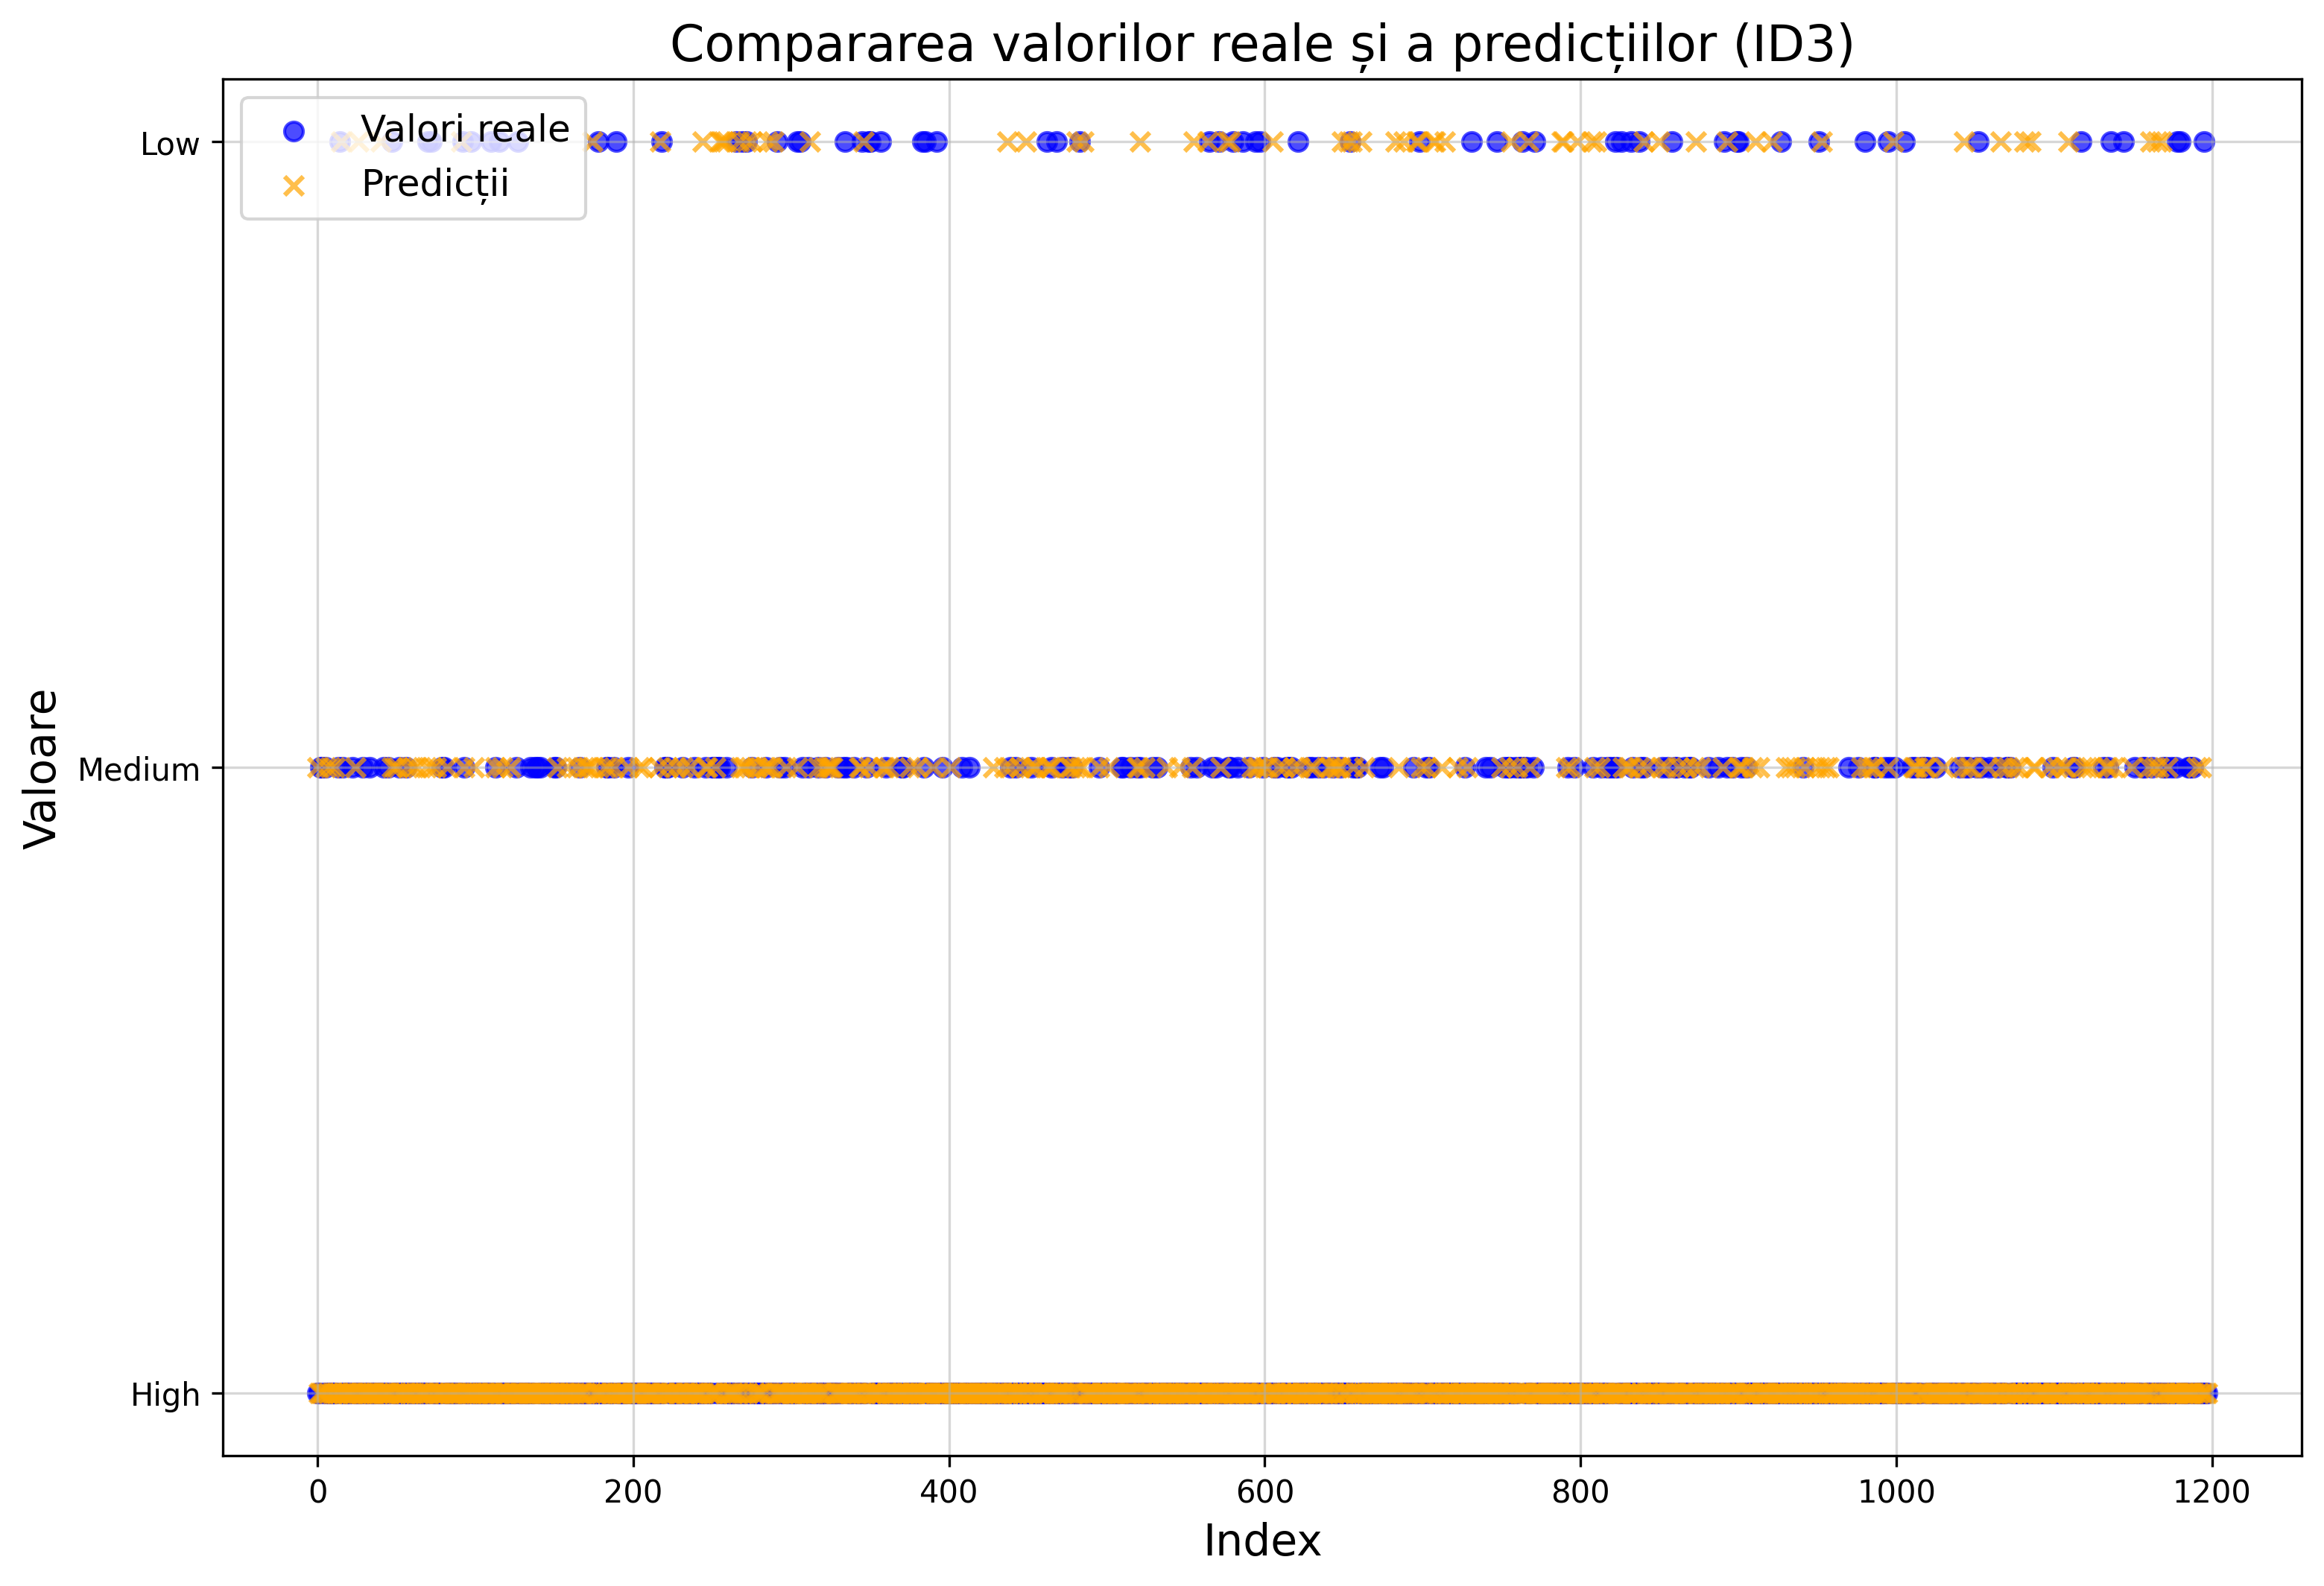
\includegraphics[width=0.8\textwidth]{img/id3_predictions.png}
\caption{ID3 - compararea rezultatelor obținute cu cele reale}
\label{fig:scatter}
\end{figure}

\begin{figure}[H]
\centering
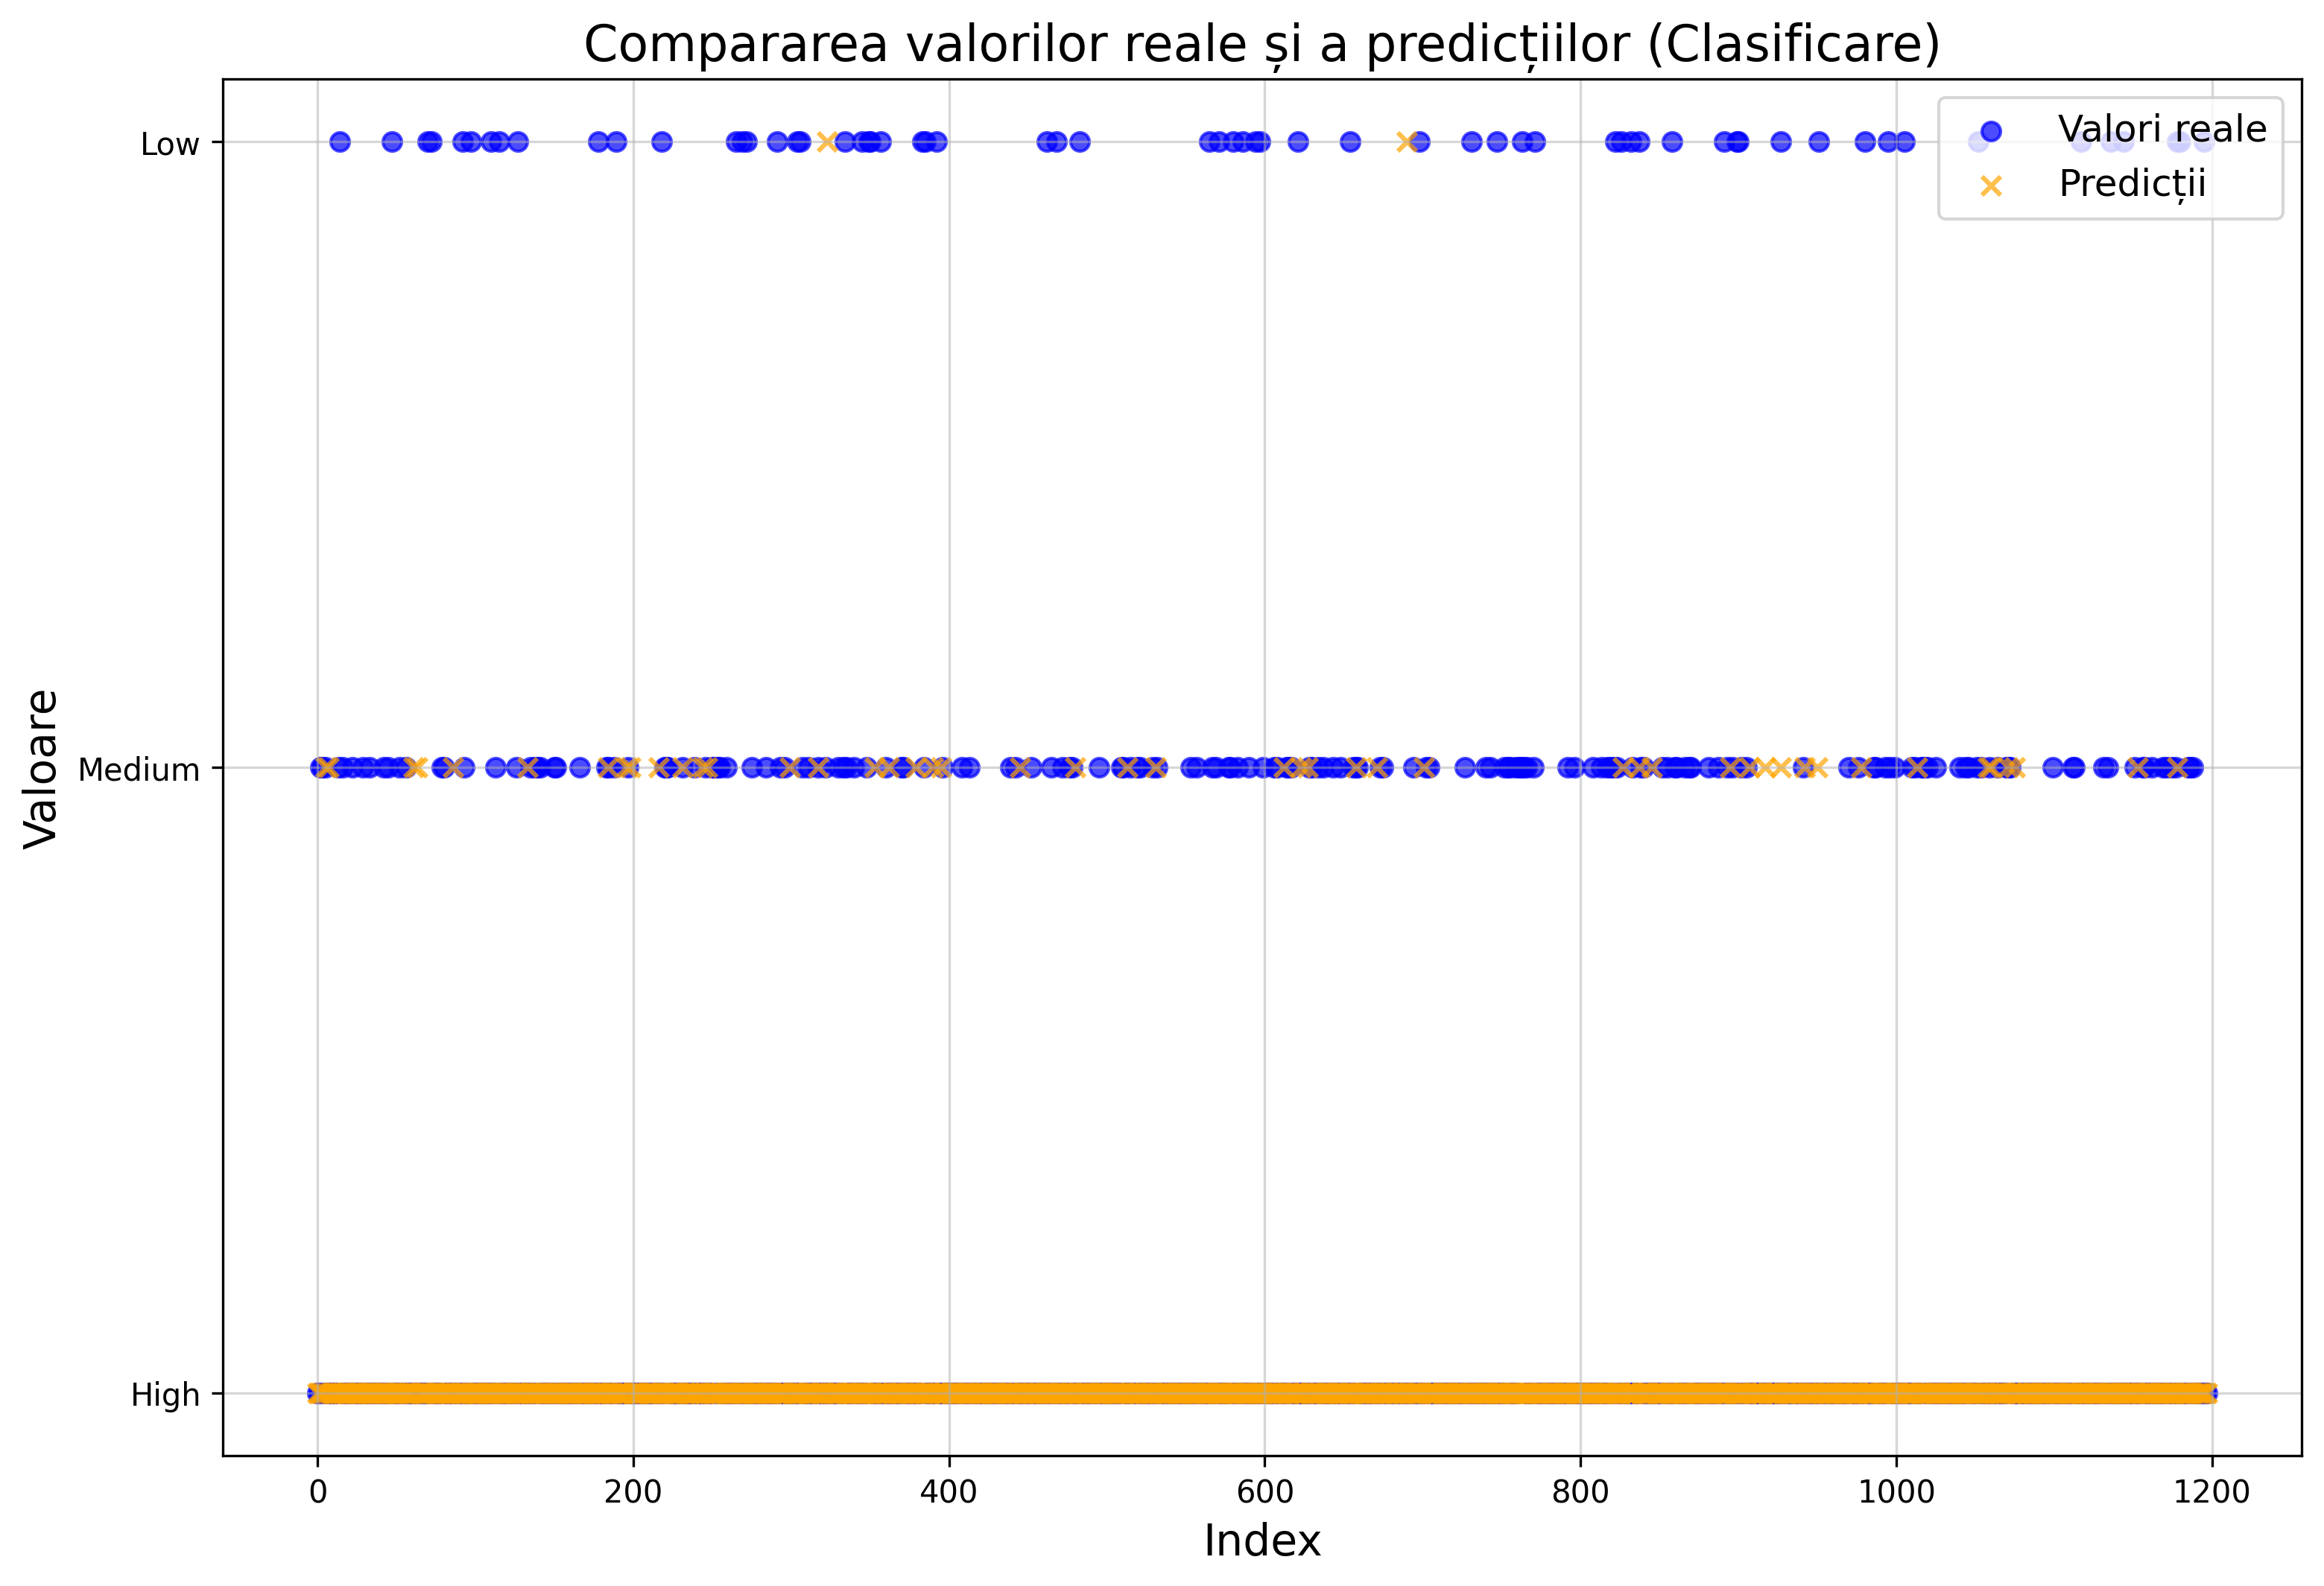
\includegraphics[width=0.8\textwidth]{img/knn_predictions.png}
\caption{kNN - compararea rezultatelor obținute cu cele reale}
\label{fig:scatter}
\end{figure}

\begin{figure}[H]
\centering
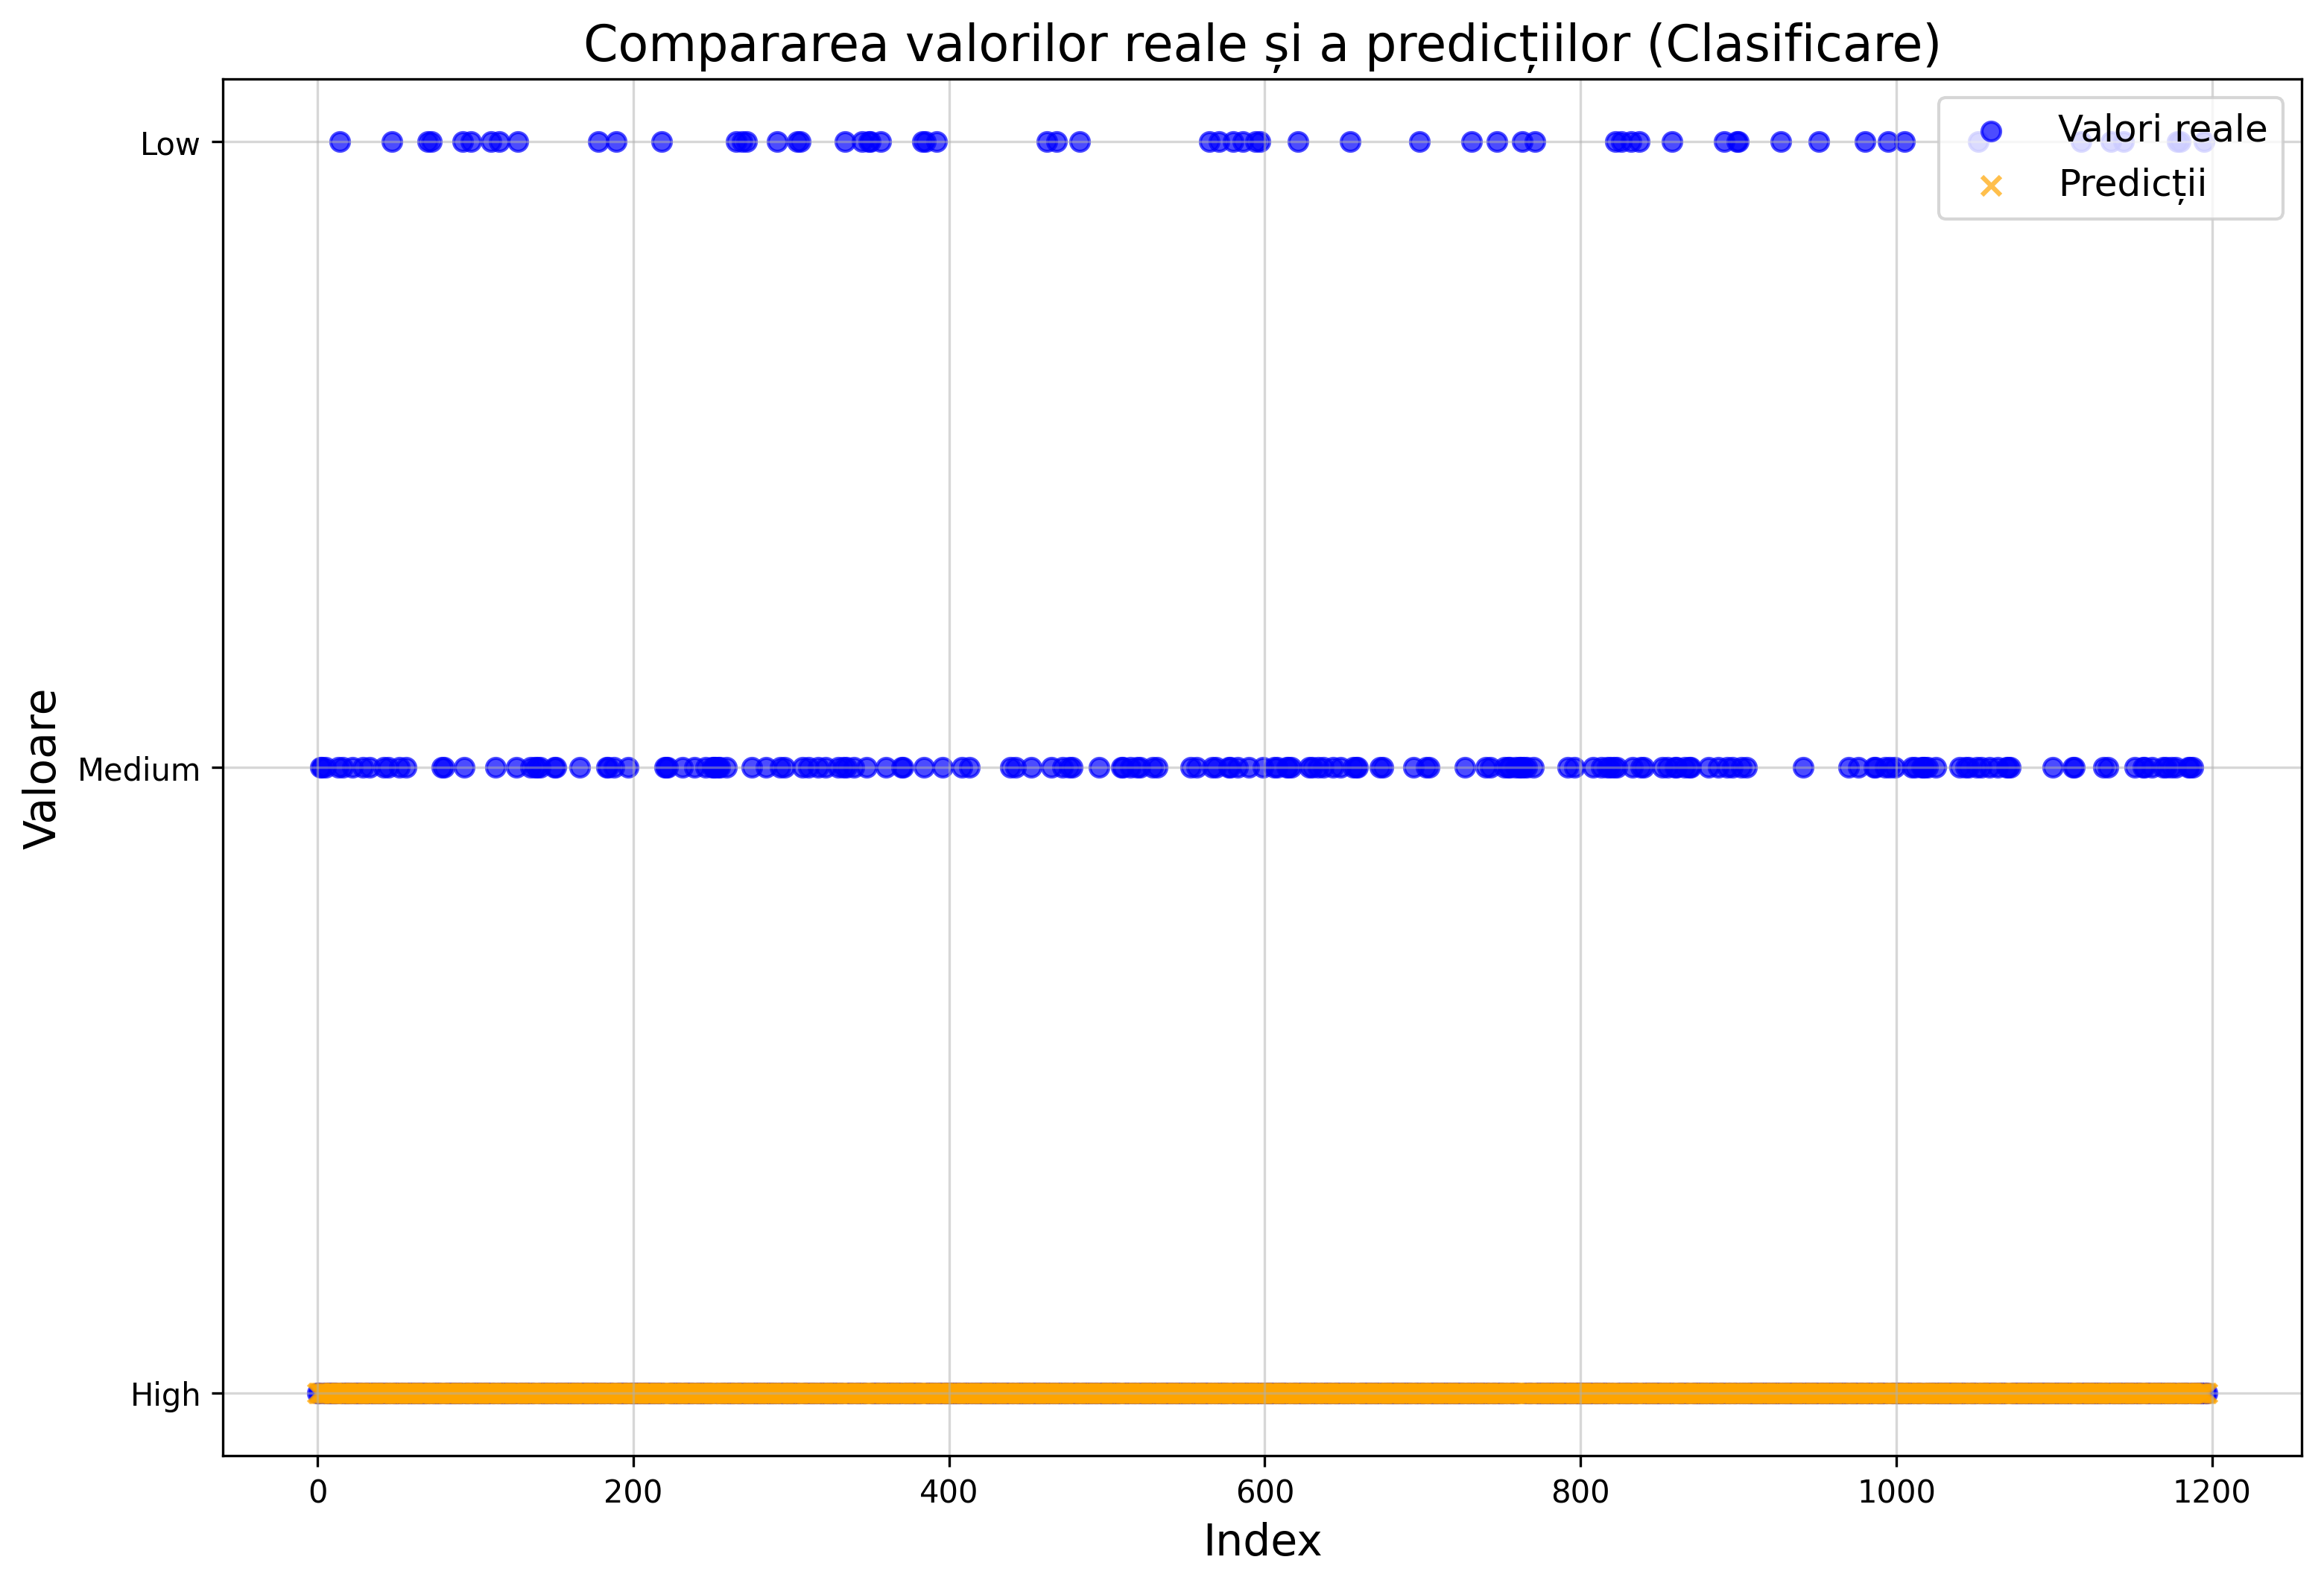
\includegraphics[width=0.8\textwidth]{img/adaboost_predictions.png}
\caption{AdaBoost - compararea rezultatelor obținute cu cele reale}
\label{fig:scatter}
\end{figure}

\subsection*{Grafice comparative}
În Figura \ref{fig:scatter}, este prezentată comparația dintre valorile reale ale profitului și cele prezise de fiecare algoritm, iar în Figura \ref{fig:pie}, se poate observa distribuția relativă a performanțelor bazate pe MSE.

\begin{figure}[H]
\centering
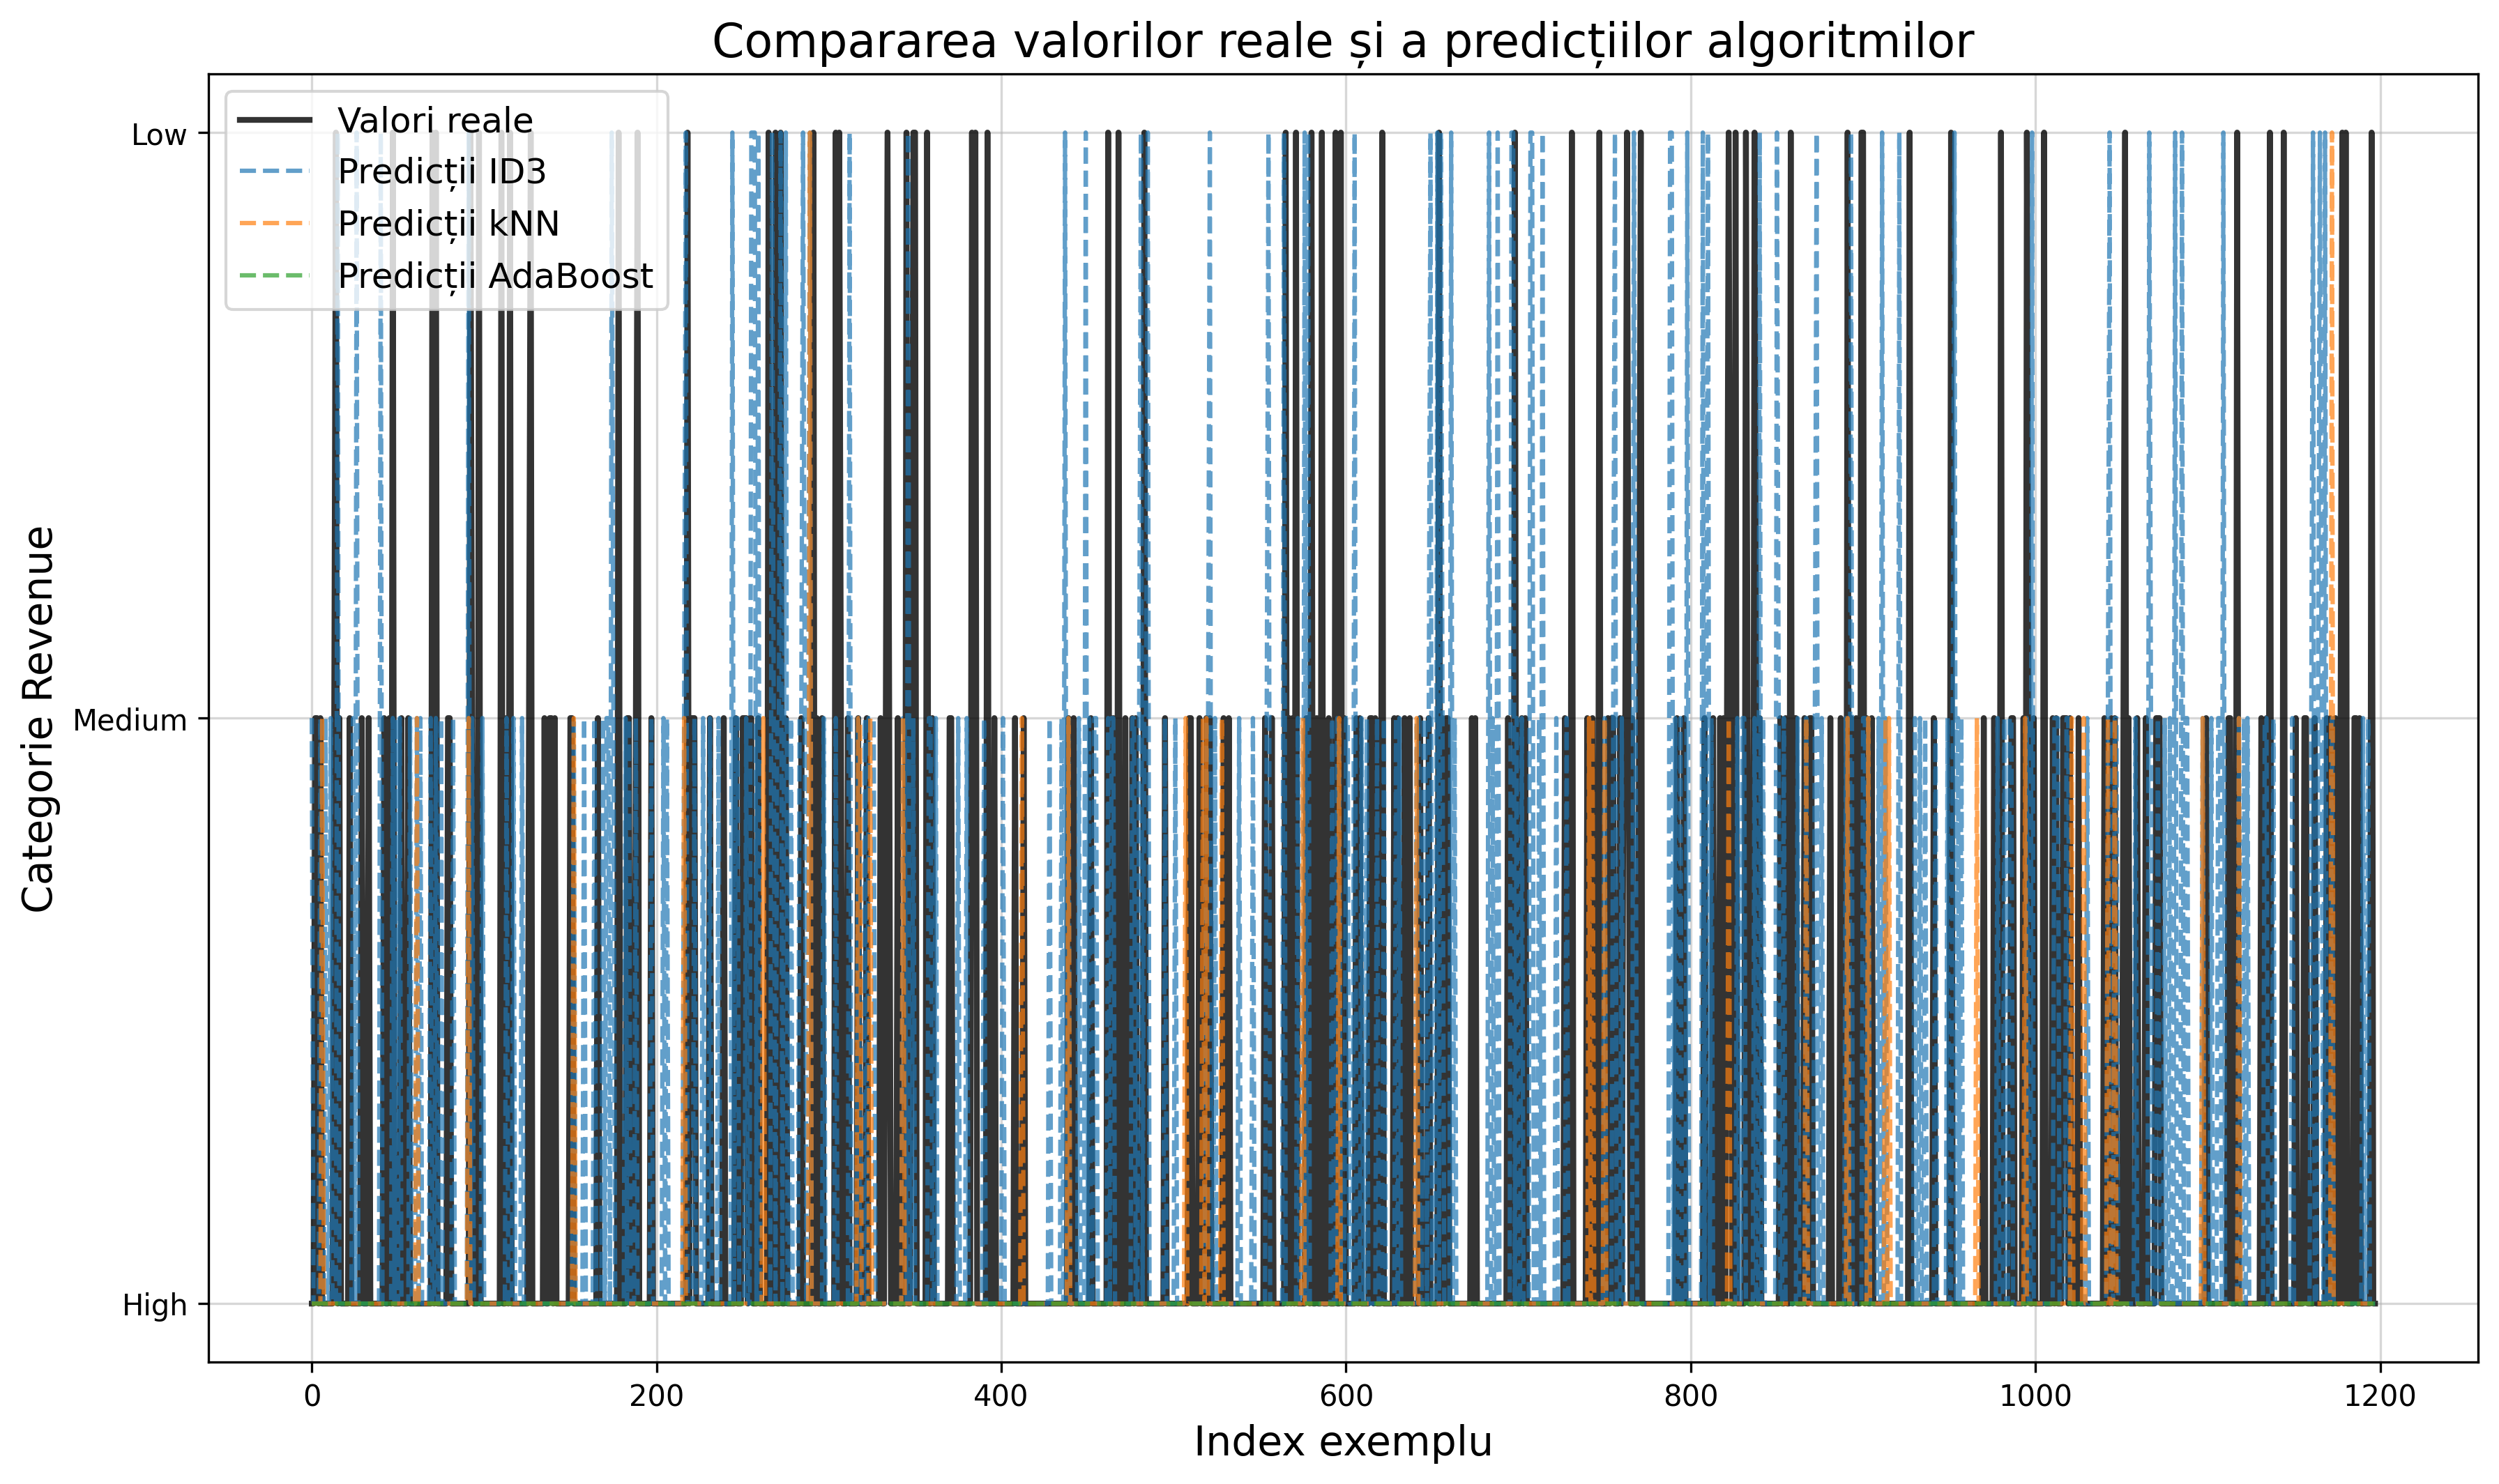
\includegraphics[width=0.8\textwidth]{img/comparative_graph.png}
\caption{Comparația între valorile reale și cele prezise de algoritmi.}
\label{fig:scatter}
\end{figure}

\begin{figure}[H]
\centering
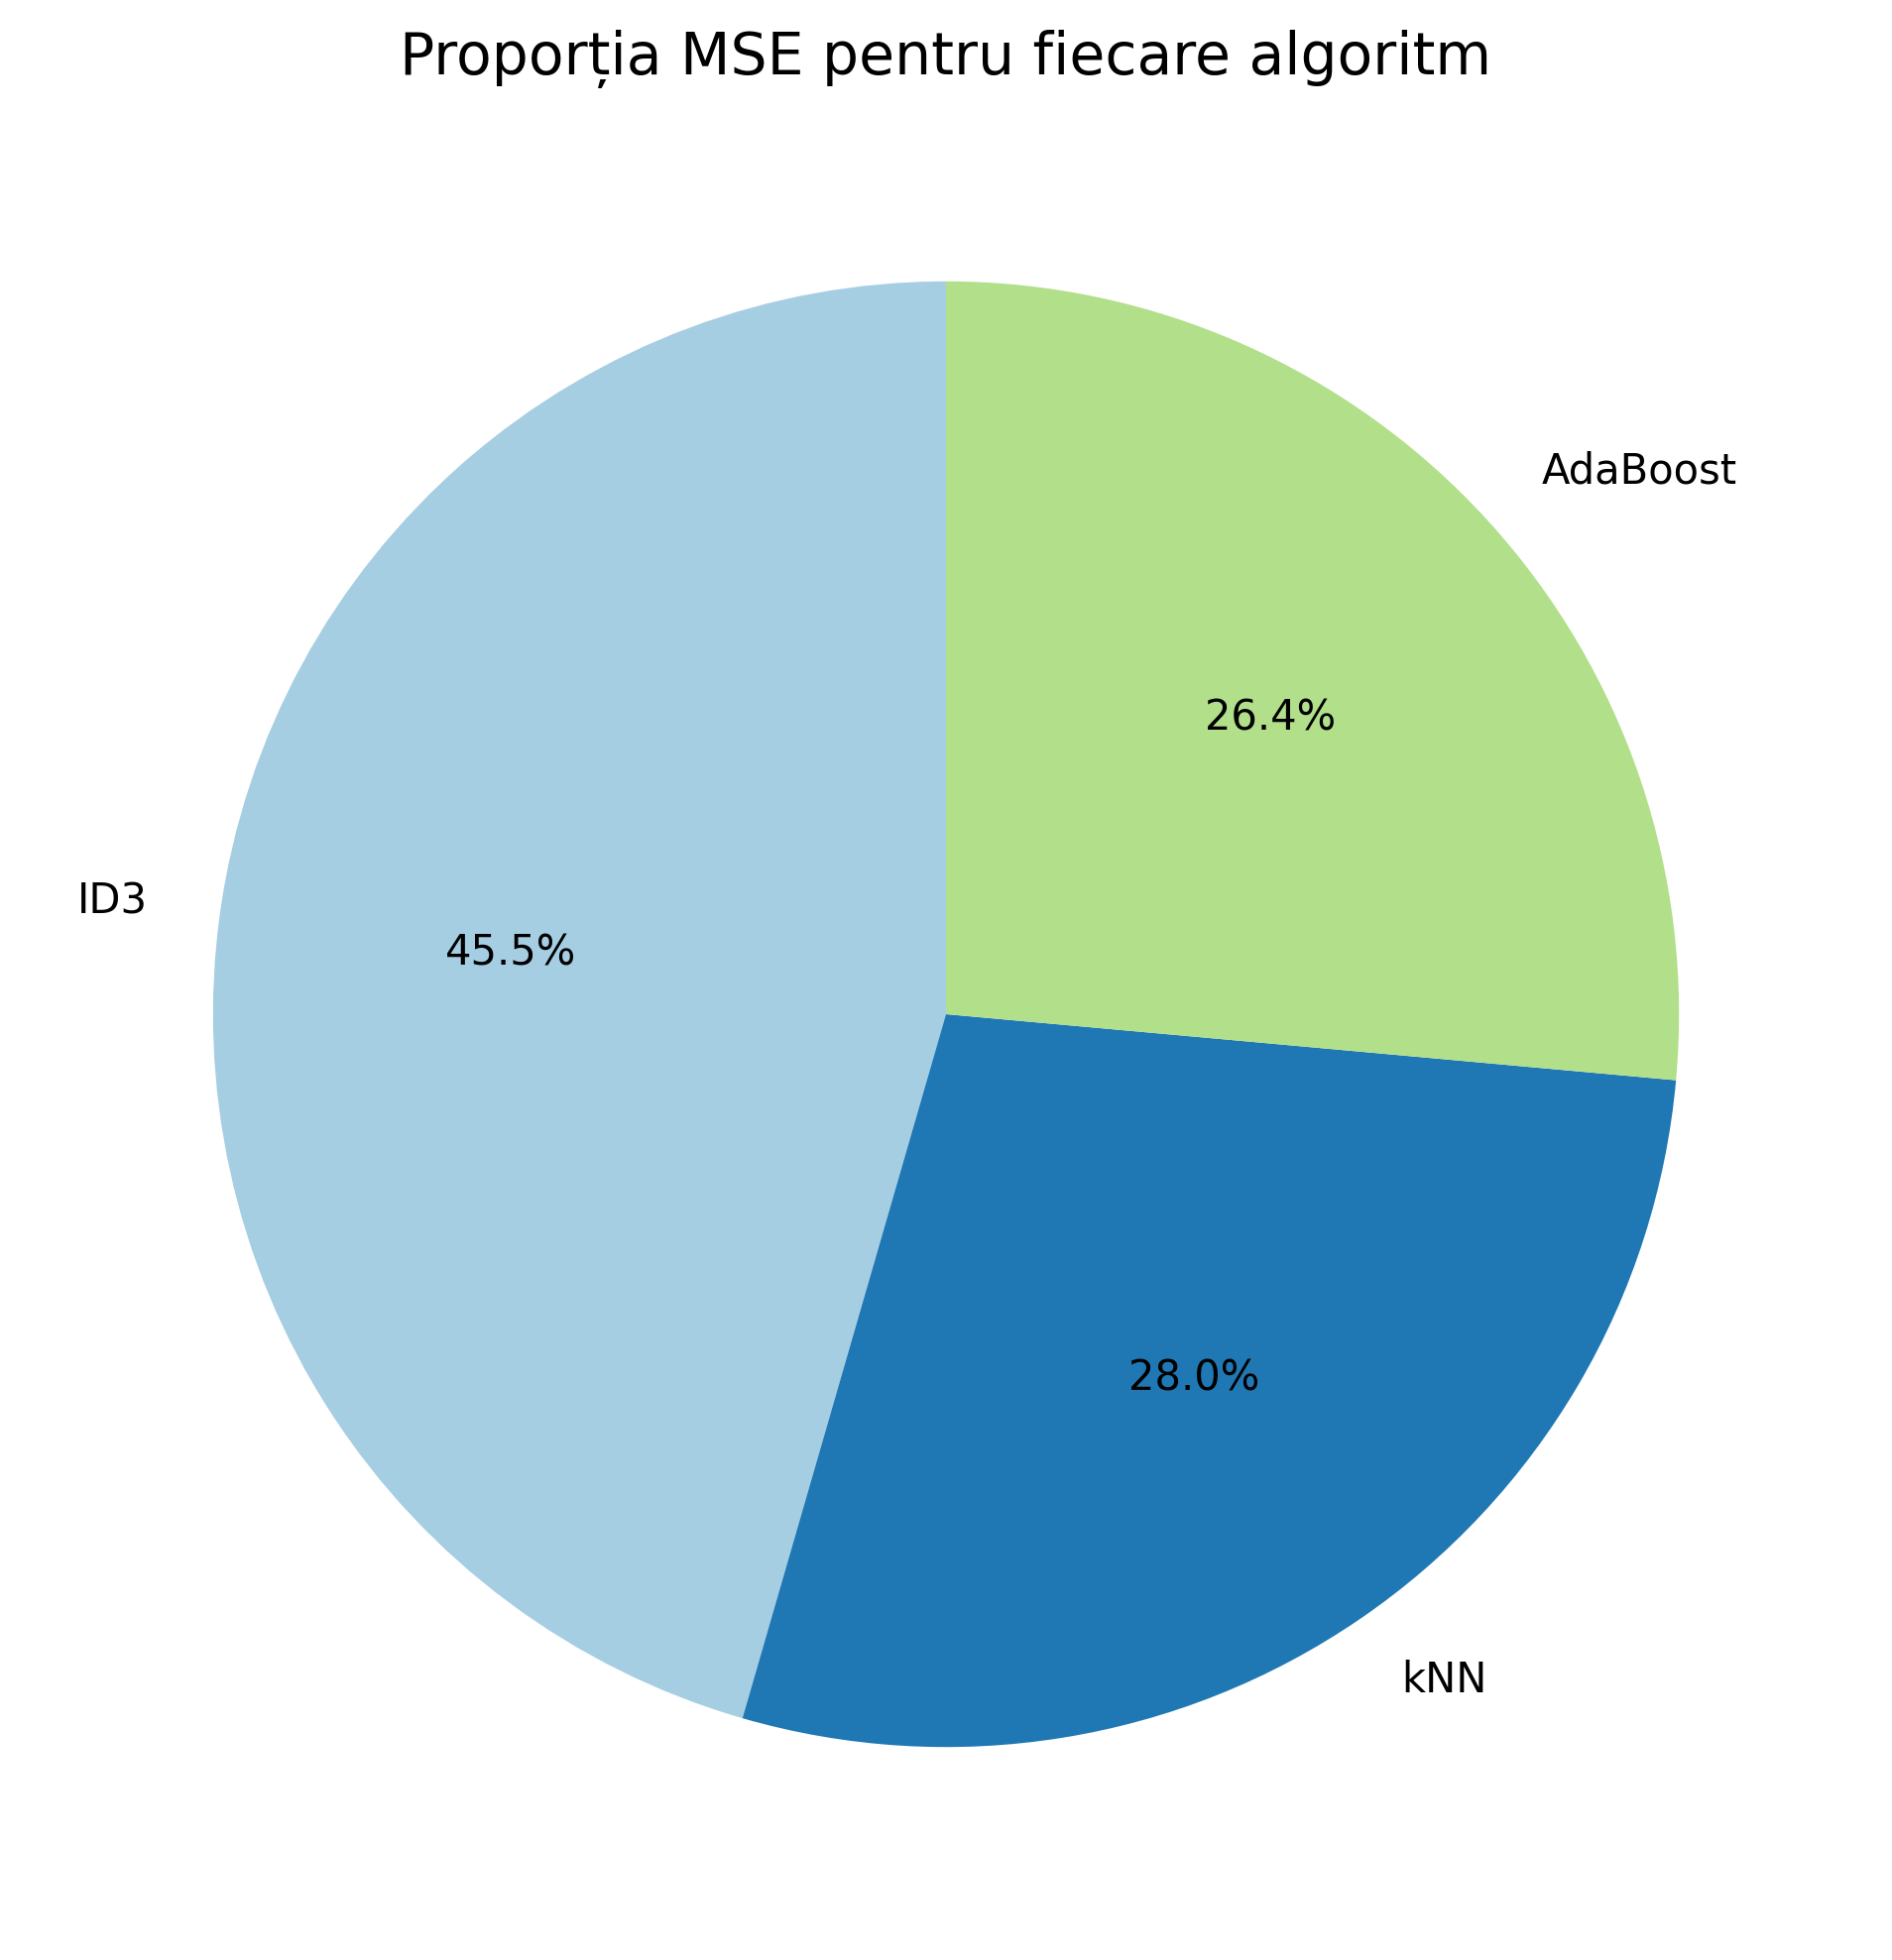
\includegraphics[width=0.6\textwidth]{img/mse_pie_chart.png}
\caption{Distribuția performanței algoritmilor în funcție de MSE}
\label{fig:pie}
\end{figure}

\subsection*{Concluzie}
Deși algoritmul AdaBoost a obținut cele mai bune rezultate, alegerea finală a algoritmului depinde de echilibrul dintre interpretabilitate, complexitate și performanță. kNN rămâne o opțiune viabilă pentru scenarii mai puțin complexe, în timp ce ID3 poate fi utilizat pentru înțelegerea relațiilor dintre variabile.

\end{document}
